\documentclass{standalone}
\usepackage{tikz}
\usepackage{ctex,siunitx,ninecolors}
\usepackage{tkz-euclide}
\usepackage{amsmath}
\usetikzlibrary{patterns, calc}
\usetikzlibrary {decorations.pathmorphing, decorations.pathreplacing, decorations.shapes,}
\begin{document}
\small
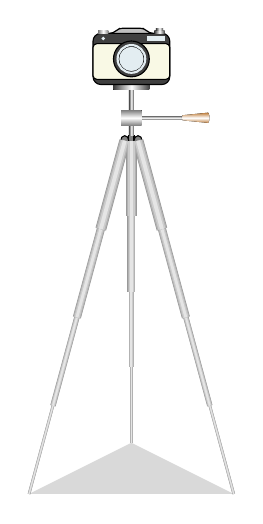
\begin{tikzpicture}[>=stealth,scale=0.65]
  \fill[lightgray!60](-2,0)--(2,0)--(0,1);
  \fill[gray](-0.13,6.8)rectangle(0.13,7);
  \draw[fill=gray](0.05,6.8)rectangle(-0.05,7);
  \draw[fill=gray](0.13,6.9)ellipse(0.08 and 0.1);
  \draw[fill=gray](-0.13,6.9)ellipse(0.08 and 0.1);
  \foreach \x[count =\i] in {4,3,2,1}
  {
    \foreach \w in {80,60,40,20}
    {
      \draw[line width={\i*sin(\w)},gray!\w](0,6.9)--(0,6.9-5.9/4*\x);
      \draw[line width={\i*sin(\w)},gray!\w](0.13,6.9)--(1.87/4*\x+0.13,-6.9/4*\x+6.9);
      \draw[line width={\i*sin(\w)},gray!\w](-0.13,6.9)--(-1.87/4*\x-0.13,-6.9/4*\x+6.9);
    }
  }
  \fill[left color=darkgray,right color=darkgray,middle color=white]
  (-0.05,8)rectangle(0.05,7);
  \fill[top color=gray,bottom color=gray,middle color=white](0,7.32)rectangle(1,7.38);
  \fill[top color=brown,bottom color=brown,middle color=white](1,7.3)to[bend left](1,7.4)--(1.5,7.45)to[bend left](1.5,7.25)--cycle;
  \fill[top color=gray,bottom color=gray,middle color=white](-0.2,7.2)rectangle(0.2,7.5);
  %%% 相机
  \fill[left color=darkgray,right color=darkgray,middle color=white](-0.35,7.9)rectangle(0.35,8);
  \draw[fill=lightgray,rounded corners=0.5mm](-0.55,9)--(-0.35,9)--(-0.25,9.1)--(0.25,9.1)--(0.35,9)--(0.55,9);
  \draw[rounded corners=1mm,fill=darkgray](-0.75,8)rectangle(0.75,9);
  \draw[fill=yellow9!20,rounded corners=0.5mm](-0.75,8.1)rectangle(0.75,8.8);
  \draw[fill=darkgray](0,8.5)circle(0.35);
  \draw[fill=cyan!20!lightgray!30](0,8.5)circle(0.25);
  \draw[cyan!20!lightgray!30,thick](0,8.5)circle(0.27);
  \fill[cyan!20!lightgray!30](0.3,8.85)rectangle(0.65,8.95);
  \fill[cyan!20!lightgray!30](-0.55,8.9)circle(1pt);
  \fill[left color=gray,right color=gray,middle color=white](-0.65,9)rectangle(-0.45,9.05);
  \fill[left color=darkgray,right color=darkgray,middle color=white](0.65,9)rectangle(0.45,9.05);
  \fill[left color=darkgray,right color=darkgray,middle color=white](0.62,9.1)rectangle(0.48,9.05);

\end{tikzpicture}
\end{document}